% Week 09: Game Loop Pattern & Singleton Pattern
% Complete Presentation for Overleaf
% Compile with: pdflatex week09-presentation.tex

\documentclass[aspectratio=169]{beamer}
\usepackage{tikz}
\usepackage{pgfplots}
\usepackage{listings}
\usepackage{xcolor}
\usepackage{fontawesome5}

\usetikzlibrary{positioning,shapes,arrows,calc,decorations.pathreplacing,fit}
\pgfplotsset{compat=1.18}

% Theme
\usetheme{Madrid}
\usecolortheme{default}

% Custom colors
\definecolor{problemred}{RGB}{220,50,50}
\definecolor{solutiongreen}{RGB}{50,150,50}
\definecolor{codeblue}{RGB}{0,100,200}

% Code listing style
\lstset{
    language=Java,
    basicstyle=\ttfamily\small,
    keywordstyle=\color{blue}\bfseries,
    commentstyle=\color{gray}\itshape,
    stringstyle=\color{red},
    numbers=left,
    numberstyle=\tiny\color{gray},
    stepnumber=1,
    frame=single,
    breaklines=true,
    captionpos=b,
    showstringspaces=false
}

% Title page
\title[Week 09: Game Loop \& Singleton]{Week 09: Design Patterns in Game Development}
\subtitle{Game Loop Pattern \& Singleton Pattern}
\author{OOP Course}
\date{\today}

\begin{document}

% ============================================================================
% TITLE SLIDE
% ============================================================================
\begin{frame}
    \titlepage
\end{frame}

% ============================================================================
% TABLE OF CONTENTS
% ============================================================================
\begin{frame}{Agenda}
    \tableofcontents
\end{frame}

% ============================================================================
% SECTION 1: INTRODUCTION
% ============================================================================
\section{Introduction}

\begin{frame}{Learning Journey}
    \begin{block}{Progressive Learning Approach}
        This week demonstrates \textbf{real-world software evolution}:
        \begin{itemize}
            \item Start simple (works!)
            \item Add features (problems emerge!)
            \item Apply patterns (problems solved!)
            \item \textbf{Maintain solutions} (no regression!)
        \end{itemize}
    \end{block}

    \vspace{0.5cm}

    \begin{center}
        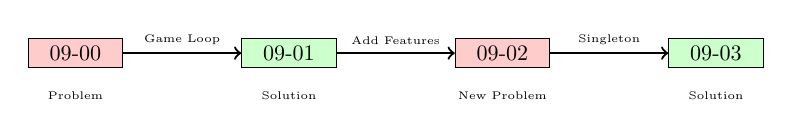
\begin{tikzpicture}[node distance=1.5cm, scale=0.8, every node/.style={scale=0.8}]
            \node[rectangle, draw, fill=red!20, minimum width=1.5cm] (b00) {09-00};
            \node[rectangle, draw, fill=green!20, minimum width=1.5cm, right=of b00] (b01) {09-01};
            \node[rectangle, draw, fill=red!20, minimum width=1.5cm, right=of b01] (b02) {09-02};
            \node[rectangle, draw, fill=green!20, minimum width=1.5cm, right=of b02] (b03) {09-03};

            \draw[->,thick] (b00) -- (b01) node[midway,above,font=\tiny] {Game Loop};
            \draw[->,thick] (b01) -- (b02) node[midway,above,font=\tiny] {Add Features};
            \draw[->,thick] (b02) -- (b03) node[midway,above,font=\tiny] {Singleton};

            \node[below=0.2cm of b00,font=\tiny] {Problem};
            \node[below=0.2cm of b01,font=\tiny] {Solution};
            \node[below=0.2cm of b02,font=\tiny] {New Problem};
            \node[below=0.2cm of b03,font=\tiny] {Solution};
        \end{tikzpicture}
    \end{center}
\end{frame}

% ============================================================================
% SECTION 2: BRANCH 09-00
% ============================================================================
\section{Branch 09-00: The Problem}

\begin{frame}{09-00: Monolithic Anti-Pattern}
    \begin{columns}[T]
        \begin{column}{0.5\textwidth}
            \textbf{\textcolor{problemred}{Problems Demonstrated:}}
            \begin{itemize}
                \item[\faTimesCircle] Frame rate coupling (2 FPS!)
                \item[\faTimesCircle] Untestable code
                \item[\faTimesCircle] Flickering display
                \item[\faTimesCircle] 150+ lines in main()
                \item[\faTimesCircle] Poor maintainability
            \end{itemize}

            \vspace{0.5cm}

            \begin{alertblock}{Intentionally Bad!}
                This code demonstrates anti-patterns for educational purposes.
            \end{alertblock}
        \end{column}

        \begin{column}{0.5\textwidth}
            \begin{center}
                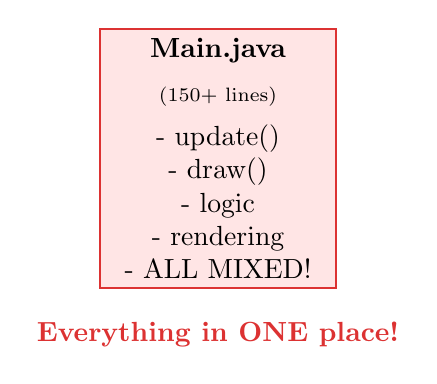
\begin{tikzpicture}[scale=0.7]
                    \node[rectangle, draw=problemred, thick, minimum width=3cm, minimum height=2cm, fill=red!10, align=center] (main) {
                        \textbf{Main.java} \\[4pt]
                        \scriptsize (150+ lines) \\[4pt]
                        - update() \\
                        - draw() \\
                        - logic \\
                        - rendering \\
                        - ALL MIXED!
                    };

                    \node[below=0.3cm of main, text=problemred, font=\bfseries] {Everything in ONE place!};
                \end{tikzpicture}
            \end{center}
        \end{column}
    \end{columns}
\end{frame}

\begin{frame}[fragile]{09-00: Code Example}
\begin{lstlisting}[caption={Monolithic main() method}]
public static void main(String[] args) {
    // ALL IN ONE METHOD!
    while (running) {
        // Update logic
        npc.x += npc.velocity;

        // Render (causes slowdown!)
        clearScreen();
        drawGrid();
        drawNPC();

        // Slow! Couples logic to render speed
        Thread.sleep(100); // 10 FPS max
    }
}
\end{lstlisting}

\begin{alertblock}{Problem}
    Update and render are \textbf{mixed together}. Slow rendering = slow game logic!
\end{alertblock}
\end{frame}

% ============================================================================
% SECTION 3: BRANCH 09-01
% ============================================================================
\section{Branch 09-01: Game Loop Pattern}

\begin{frame}{09-01: Game Loop Pattern Solution}
    \begin{columns}[T]
        \begin{column}{0.5\textwidth}
            \textbf{\textcolor{solutiongreen}{Solutions Implemented:}}
            \begin{itemize}
                \item[\faCheckCircle] Separated update() \& draw()
                \item[\faCheckCircle] Delta time (frame-independent!)
                \item[\faCheckCircle] 100\% testable
                \item[\faCheckCircle] Selective rendering (no flicker)
                \item[\faCheckCircle] 60 FPS stable
            \end{itemize}

            \vspace{0.5cm}

            \begin{exampleblock}{Result}
                \textbf{30x performance improvement!} \\
                2 FPS → 60 FPS
            \end{exampleblock}
        \end{column}

        \begin{column}{0.5\textwidth}
            \begin{center}
                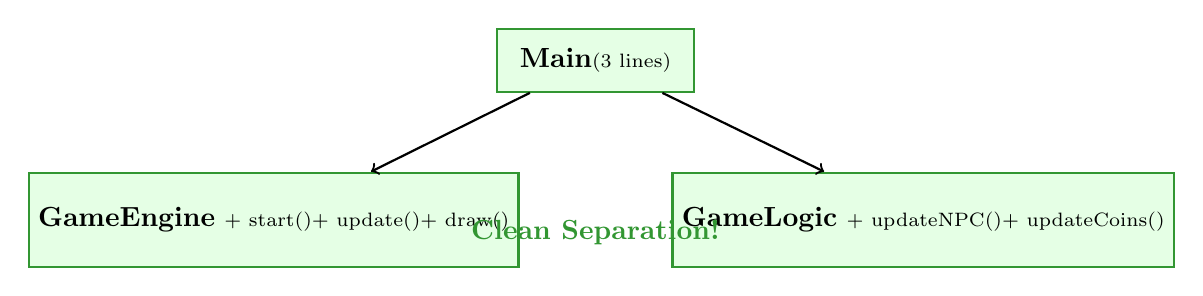
\begin{tikzpicture}[scale=0.6]
                    \node[rectangle, draw=solutiongreen, thick, minimum width=2.5cm, minimum height=0.8cm, fill=green!10] (main) {\textbf{Main} \\ \scriptsize (3 lines)};

                    \node[rectangle, draw=solutiongreen, thick, minimum width=2.5cm, minimum height=1.2cm, fill=green!10, below left=1cm and -0.3cm of main] (engine) {
                        \textbf{GameEngine} \\[2pt]
                        \scriptsize + start() \\
                        \scriptsize + update() \\
                        \scriptsize + draw()
                    };

                    \node[rectangle, draw=solutiongreen, thick, minimum width=2.5cm, minimum height=1.2cm, fill=green!10, below right=1cm and -0.3cm of main] (logic) {
                        \textbf{GameLogic} \\[2pt]
                        \scriptsize + updateNPC() \\
                        \scriptsize + updateCoins()
                    };

                    \draw[->,thick] (main) -- (engine);
                    \draw[->,thick] (main) -- (logic);

                    \node[below=1.5cm of main, text=solutiongreen, font=\bfseries] {Clean Separation!};
                \end{tikzpicture}
            \end{center}
        \end{column}
    \end{columns}
\end{frame}

\begin{frame}[fragile]{09-01: Game Loop Implementation}
\begin{lstlisting}[caption={Proper game loop structure}]
public void start() {
    running = true;
    long lastTime = System.nanoTime();

    while (running) {
        // Calculate delta time
        float delta = (currentTime - lastTime) / 1e9f;
        lastTime = currentTime;

        update(delta);  // LOGIC ONLY
        draw();         // RENDERING ONLY
        sync();         // FPS CONTROL
    }
}
\end{lstlisting}

\begin{block}{Key Benefits}
    \begin{itemize}
        \item \textbf{update()}: Pure logic, no rendering → \textcolor{solutiongreen}{Testable!}
        \item \textbf{draw()}: Pure rendering, no logic → \textcolor{solutiongreen}{Fast!}
        \item \textbf{Delta time}: Frame-rate independent → \textcolor{solutiongreen}{Consistent!}
    \end{itemize}
\end{block}
\end{frame}

\begin{frame}{09-01: Delta Time Explanation}
    \begin{block}{Problem Without Delta Time}
        Different frame rates → Different game speeds!
    \end{block}

    \vspace{0.3cm}

    \begin{center}
        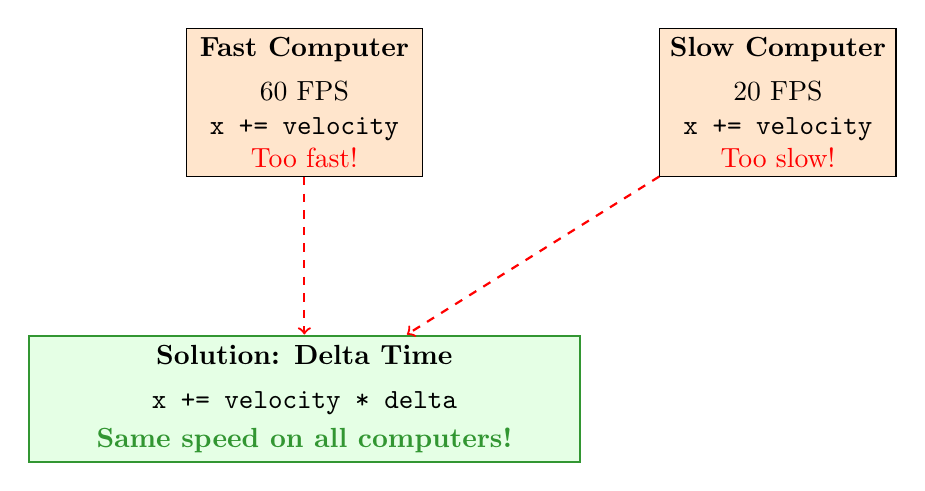
\begin{tikzpicture}[scale=0.9]
            % Fast computer
            \node[rectangle, draw, fill=orange!20, minimum width=3cm, minimum height=1.5cm, align=center] (fast) {
                \textbf{Fast Computer} \\[4pt]
                60 FPS \\
                \texttt{x += velocity} \\
                \textcolor{red}{Too fast!}
            };

            % Slow computer
            \node[rectangle, draw, fill=orange!20, minimum width=3cm, minimum height=1.5cm, align=center, right=3cm of fast] (slow) {
                \textbf{Slow Computer} \\[4pt]
                20 FPS \\
                \texttt{x += velocity} \\
                \textcolor{red}{Too slow!}
            };

            \node[below=2cm of fast, rectangle, draw=solutiongreen, thick, fill=green!10, minimum width=7cm, minimum height=1.5cm, align=center] (solution) {
                \textbf{Solution: Delta Time} \\[4pt]
                \texttt{x += velocity * delta} \\[2pt]
                \textcolor{solutiongreen}{\textbf{Same speed on all computers!}}
            };

            \draw[->,thick,red,dashed] (fast) -- (solution);
            \draw[->,thick,red,dashed] (slow) -- (solution);
        \end{tikzpicture}
    \end{center}
\end{frame}

\begin{frame}{09-01: Industry Usage}
    \begin{block}{This Pattern is EVERYWHERE!}
        \begin{itemize}
            \item \textbf{Unity}: \texttt{Update()} vs \texttt{FixedUpdate()}
            \item \textbf{Unreal Engine}: \texttt{Tick(DeltaTime)}
            \item \textbf{Godot}: \texttt{\_process(delta)}
            \item \textbf{LibGDX}: \texttt{render(delta)}
            \item \textbf{Every professional game engine!}
        \end{itemize}
    \end{block}

    \vspace{0.5cm}

    \begin{exampleblock}{Key Takeaway}
        Game Loop Pattern is the \textbf{foundation of game development}.
        Master this, and you understand how ALL games work!
    \end{exampleblock}
\end{frame}

% ============================================================================
% SECTION 4: BRANCH 09-02
% ============================================================================
\section{Branch 09-02: New Problems Emerge}

\begin{frame}{09-02: Adding Features Reveals Problems}
    \begin{block}{Game Evolution}
        \textbf{09-01} worked perfectly for simple game! \\
        But when we add features (score, HUD, time tracking)... \\
        \textcolor{problemred}{\textbf{NEW problems appear!}}
    \end{block}

    \vspace{0.3cm}

    \begin{columns}[T]
        \begin{column}{0.5\textwidth}
            \textbf{New Features Added:}
            \begin{itemize}
                \item Score tracking
                \item HUD display
                \item Game time
                \item Level management
            \end{itemize}

            \vspace{0.3cm}

            \textbf{Requirement:}
            \begin{itemize}
                \item Multiple components need to access \textbf{same data}
                \item Need global state management!
            \end{itemize}
        \end{column}

        \begin{column}{0.5\textwidth}
            \textbf{\textcolor{problemred}{NEW Problems:}}
            \begin{itemize}
                \item[\faTimesCircle] Multiple GameManager instances
                \item[\faTimesCircle] Object drilling (4 levels!)
                \item[\faTimesCircle] State inconsistency (HUD bug!)
                \item[\faTimesCircle] No compile-time protection
            \end{itemize}

            \vspace{0.3cm}

            \begin{alertblock}{Key Insight}
                Current design doesn't \textbf{scale}!
            \end{alertblock}
        \end{column}
    \end{columns}
\end{frame}

\begin{frame}{09-02: The Bug Demonstrated}
    \begin{center}
        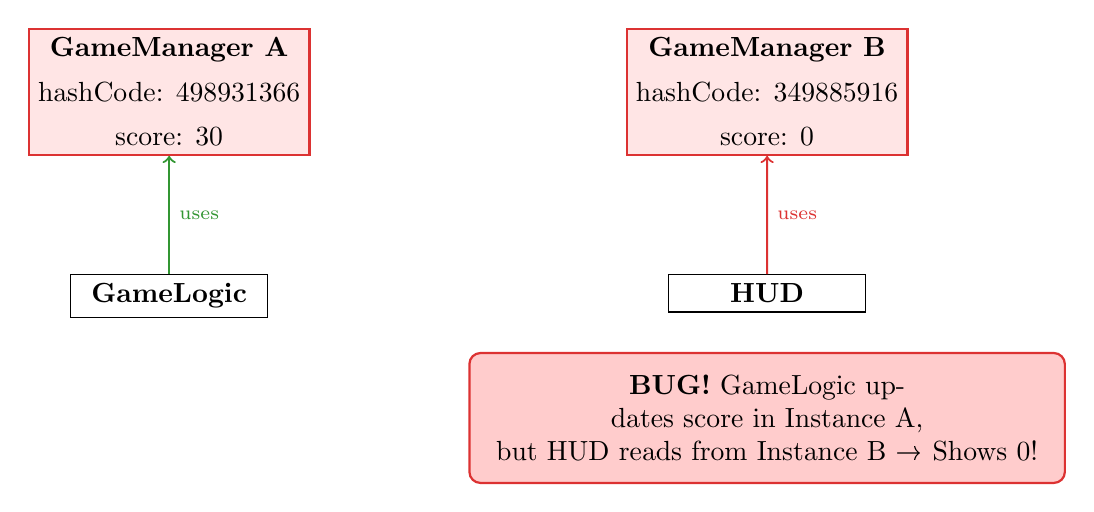
\begin{tikzpicture}[scale=0.8]
            % Instance A
            \node[rectangle, draw=problemred, thick, fill=red!10, minimum width=3cm, minimum height=1.5cm, align=center] (instanceA) {
                \textbf{GameManager A} \\[4pt]
                hashCode: 498931366 \\[4pt]
                score: 30
            };

            % Instance B
            \node[rectangle, draw=problemred, thick, fill=red!10, minimum width=3cm, minimum height=1.5cm, align=center, right=4cm of instanceA] (instanceB) {
                \textbf{GameManager B} \\[4pt]
                hashCode: 349885916 \\[4pt]
                score: 0
            };

            % GameLogic uses A
            \node[below=1.5cm of instanceA, rectangle, draw, minimum width=2.5cm] (logic) {\textbf{GameLogic}};
            \draw[->,thick,solutiongreen] (logic) -- (instanceA) node[midway,right] {\scriptsize uses};

            % HUD uses B (BUG!)
            \node[below=1.5cm of instanceB, rectangle, draw, minimum width=2.5cm] (hud) {\textbf{HUD}};
            \draw[->,thick,problemred] (hud) -- (instanceB) node[midway,right] {\scriptsize uses};

            % Bug annotation
            \node[below=0.5cm of hud, fill=red!20, draw=problemred, thick, rounded corners, inner sep=8pt, text width=7cm, align=center] {
                \textbf{BUG!} GameLogic updates score in Instance A, \\
                but HUD reads from Instance B → Shows 0!
            };
        \end{tikzpicture}
    \end{center}
\end{frame}

\begin{frame}{09-02: Object Drilling Problem}
    \begin{center}
        \scalebox{0.7}{
            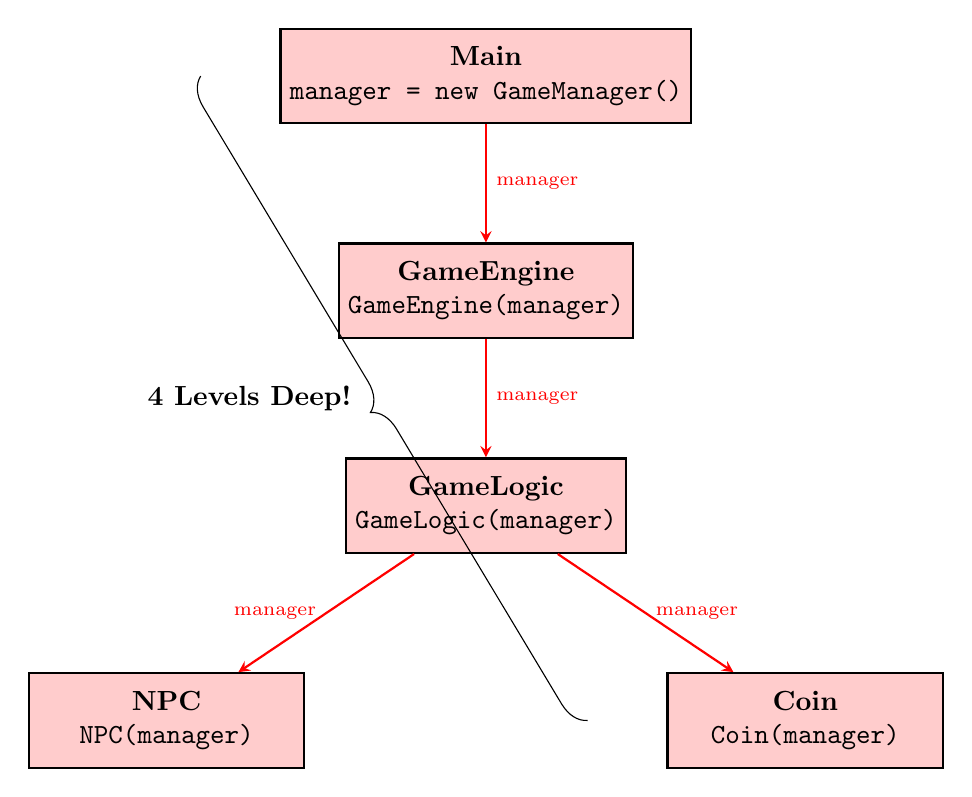
\begin{tikzpicture}[
                class/.style={rectangle, draw=black, thick, minimum width=3.5cm, minimum height=1.2cm, align=center},
                problem/.style={fill=red!20},
                arrow/.style={->,>=stealth,thick,red}
            ]
                \node[class, problem] (main) {\textbf{Main} \\ \texttt{manager = new GameManager()}};
                \node[class, problem, below=1.5cm of main] (engine) {\textbf{GameEngine} \\ \texttt{GameEngine(manager)}};
                \node[class, problem, below=1.5cm of engine] (logic) {\textbf{GameLogic} \\ \texttt{GameLogic(manager)}};
                \node[class, problem, below left=1.5cm and 0.5cm of logic] (npc) {\textbf{NPC} \\ \texttt{NPC(manager)}};
                \node[class, problem, below right=1.5cm and 0.5cm of logic] (coin) {\textbf{Coin} \\ \texttt{Coin(manager)}};

                \draw[arrow] (main) -- (engine) node[midway,right,font=\scriptsize] {manager};
                \draw[arrow] (engine) -- (logic) node[midway,right,font=\scriptsize] {manager};
                \draw[arrow] (logic) -- (npc) node[midway,left,font=\scriptsize] {manager};
                \draw[arrow] (logic) -- (coin) node[midway,right,font=\scriptsize] {manager};

                \draw[decorate,decoration={brace,amplitude=10pt,mirror}]
                    ([xshift=-1cm]main.west) -- ([xshift=-1cm]coin.west)
                    node[midway,left=12pt] {\textbf{4 Levels Deep!}};
            \end{tikzpicture}
        }
    \end{center}

    \begin{alertblock}{Problems}
        \begin{itemize}
            \item Every constructor polluted with \texttt{manager} parameter
            \item Refactoring affects 6+ files
            \item Team collaboration nightmare
        \end{itemize}
    \end{alertblock}
\end{frame}

% ============================================================================
% SECTION 5: BRANCH 09-03
% ============================================================================
\section{Branch 09-03: Singleton Pattern}

\begin{frame}{09-03: Singleton Pattern Solution}
    \begin{block}{What is Singleton?}
        A creational design pattern that ensures:
        \begin{enumerate}
            \item \textbf{Single instance}: Only ONE instance exists
            \item \textbf{Global access}: Accessible from anywhere
            \item \textbf{Lazy initialization}: Created when first needed
        \end{enumerate}
    \end{block}

    \vspace{0.3cm}

    \begin{columns}[T]
        \begin{column}{0.5\textwidth}
            \textbf{Three Components:}
            \begin{enumerate}
                \item \textcolor{red}{Private constructor}
                \item \textcolor{red}{Static instance variable}
                \item \textcolor{blue}{Public getInstance() method}
            \end{enumerate}
        \end{column}

        \begin{column}{0.5\textwidth}
            \textbf{\textcolor{solutiongreen}{Solutions:}}
            \begin{itemize}
                \item[\faCheckCircle] Single instance guaranteed
                \item[\faCheckCircle] No object drilling
                \item[\faCheckCircle] State consistency fixed
                \item[\faCheckCircle] Compile-time protection
            \end{itemize}
        \end{column}
    \end{columns}
\end{frame}

\begin{frame}[fragile]{09-03: Singleton Implementation}
\begin{lstlisting}[caption={Singleton pattern structure}]
public class GameManager {
    // 1. Static instance variable
    private static GameManager instance = null;

    // 2. Private constructor (prevents: new GameManager())
    private GameManager() {
        this.score = 0;
        // ...
    }

    // 3. Public static accessor (global access)
    public static GameManager getInstance() {
        if (instance == null) {
            instance = new GameManager();
        }
        return instance;
    }

    // Business methods
    public void addScore(int points) { /* ... */ }
}
\end{lstlisting}
\end{frame}

\begin{frame}[fragile]{09-03: Usage Comparison}
    \begin{columns}[T]
        \begin{column}{0.5\textwidth}
            \textbf{09-02: Object Drilling}
\begin{lstlisting}[basicstyle=\ttfamily\tiny]
// Main.java
GameManager mgr =
    new GameManager();
GameEngine engine =
    new GameEngine(mgr);

// GameEngine.java
public GameEngine(
    GameManager mgr) {
    this.logic =
        new GameLogic(mgr);
}

// GameLogic.java
public GameLogic(
    GameManager mgr) {
    this.mgr = mgr;
}
\end{lstlisting}
        \end{column}

        \begin{column}{0.5\textwidth}
            \textbf{09-03: Singleton}
\begin{lstlisting}[basicstyle=\ttfamily\tiny]
// Main.java
GameEngine engine =
    new GameEngine();


// GameEngine.java
public GameEngine() {
    this.logic =
        new GameLogic();
}


// GameLogic.java
public GameLogic() {
    // Access when needed:
    GameManager.getInstance()
        .addScore(10);
}
\end{lstlisting}
        \end{column}
    \end{columns}

    \vspace{0.5cm}

    \begin{exampleblock}{Result}
        \textbf{Zero} constructor parameters! Clean, simple code!
    \end{exampleblock}
\end{frame}

\begin{frame}{09-03: Singleton Solution Visualization}
    \begin{center}
        \scalebox{0.65}{
            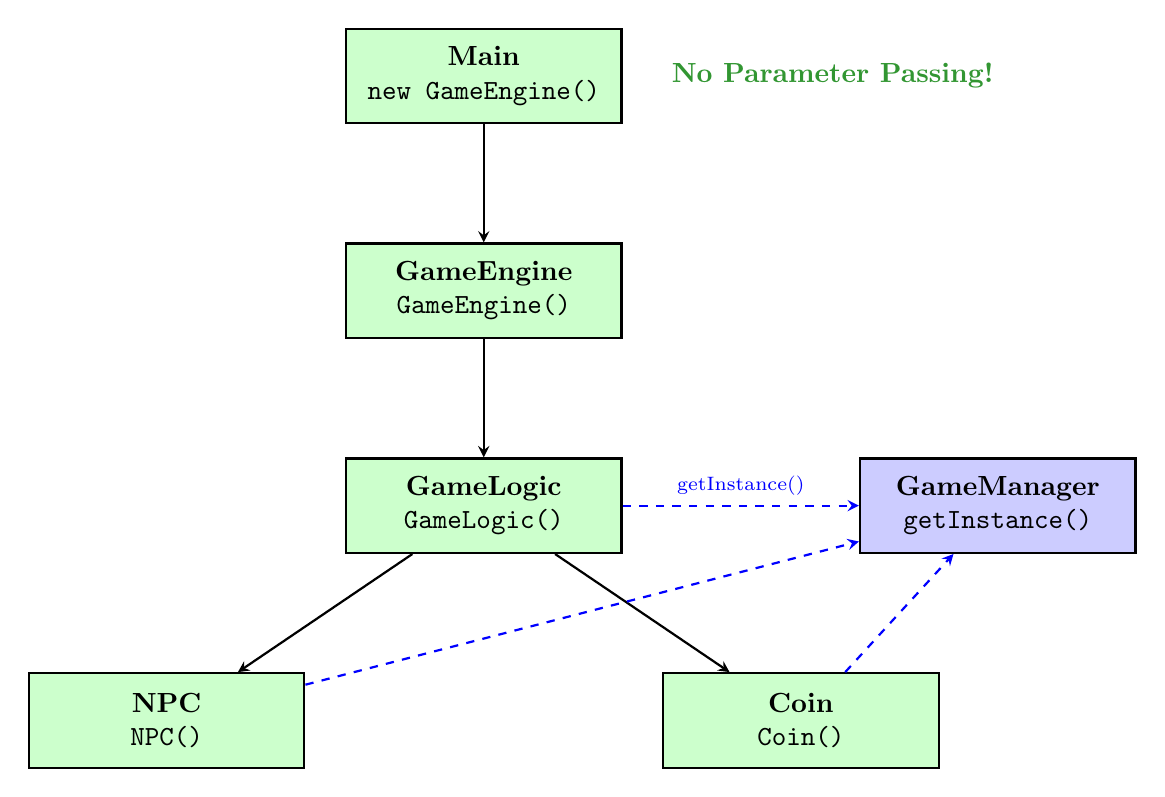
\begin{tikzpicture}[
                class/.style={rectangle, draw=black, thick, minimum width=3.5cm, minimum height=1.2cm, align=center},
                solution/.style={fill=green!20},
                singleton/.style={fill=blue!20},
                arrow/.style={->,>=stealth,thick},
                access/.style={->,>=stealth,thick,dashed,blue}
            ]
                \node[class, solution] (main) {\textbf{Main} \\ \texttt{new GameEngine()}};
                \node[class, solution, below=1.5cm of main] (engine) {\textbf{GameEngine} \\ \texttt{GameEngine()}};
                \node[class, solution, below=1.5cm of engine] (logic) {\textbf{GameLogic} \\ \texttt{GameLogic()}};
                \node[class, solution, below left=1.5cm and 0.5cm of logic] (npc) {\textbf{NPC} \\ \texttt{NPC()}};
                \node[class, solution, below right=1.5cm and 0.5cm of logic] (coin) {\textbf{Coin} \\ \texttt{Coin()}};

                \node[class, singleton, right=3cm of logic] (singleton) {\textbf{GameManager} \\ \texttt{getInstance()}};

                \draw[arrow] (main) -- (engine);
                \draw[arrow] (engine) -- (logic);
                \draw[arrow] (logic) -- (npc);
                \draw[arrow] (logic) -- (coin);

                \draw[access] (logic) -- (singleton) node[midway,above,font=\scriptsize] {getInstance()};
                \draw[access] (npc) -- (singleton);
                \draw[access] (coin) -- (singleton);

                \node[right=0.5cm of main, text=solutiongreen, font=\bfseries] {No Parameter Passing!};
            \end{tikzpicture}
        }
    \end{center}
\end{frame}

% ============================================================================
% SECTION 6: PERFORMANCE COMPARISON
% ============================================================================
\section{Performance Comparison}

\begin{frame}{Performance Metrics: FPS}
    \begin{center}
        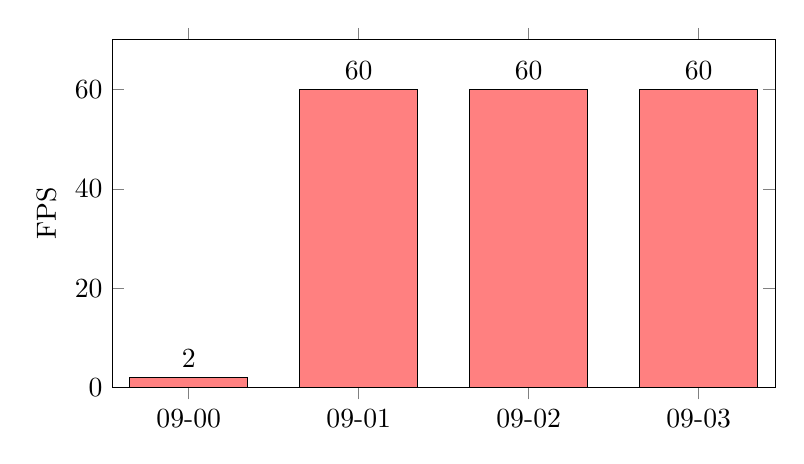
\begin{tikzpicture}
            \begin{axis}[
                ybar,
                width=10cm,
                height=6cm,
                ylabel={FPS},
                symbolic x coords={09-00,09-01,09-02,09-03},
                xtick=data,
                ymin=0,
                ymax=70,
                bar width=1.5cm,
                nodes near coords,
                enlarge x limits=0.15
            ]
                \addplot[fill=red!50] coordinates {
                    (09-00,2)
                    (09-01,60)
                    (09-02,60)
                    (09-03,60)
                };
            \end{axis}
        \end{tikzpicture}
    \end{center}

    \begin{block}{Result}
        \textbf{30x performance improvement!} (2 FPS → 60 FPS)
    \end{block}
\end{frame}

\begin{frame}{Code Quality: Lines in Main}
    \begin{center}
        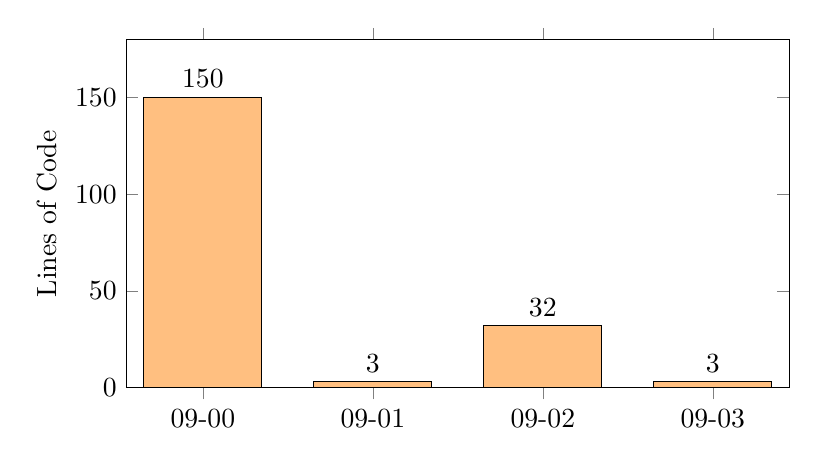
\begin{tikzpicture}
            \begin{axis}[
                ybar,
                width=10cm,
                height=6cm,
                ylabel={Lines of Code},
                symbolic x coords={09-00,09-01,09-02,09-03},
                xtick=data,
                ymin=0,
                ymax=180,
                bar width=1.5cm,
                nodes near coords,
                enlarge x limits=0.15
            ]
                \addplot[fill=orange!50] coordinates {
                    (09-00,150)
                    (09-01,3)
                    (09-02,32)
                    (09-03,3)
                };
            \end{axis}
        \end{tikzpicture}
    \end{center}

    \begin{block}{Result}
        \textbf{50x code reduction!} (150 lines → 3 lines)
    \end{block}
\end{frame}

\begin{frame}{Object Drilling Impact}
    \begin{center}
        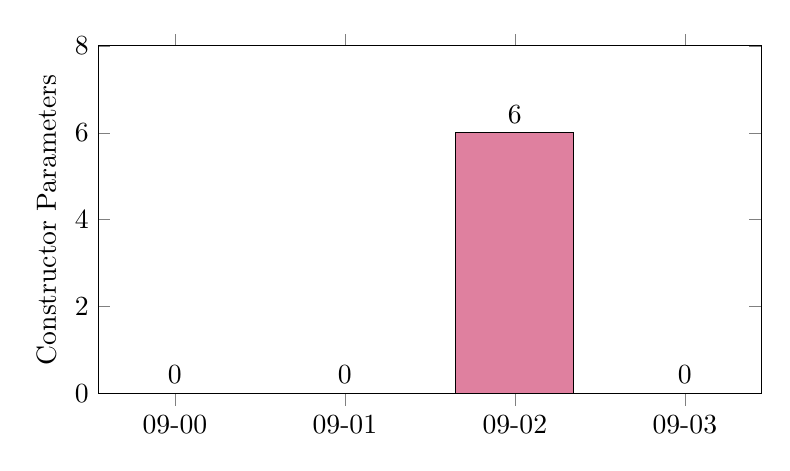
\begin{tikzpicture}
            \begin{axis}[
                ybar,
                width=10cm,
                height=6cm,
                ylabel={Constructor Parameters},
                symbolic x coords={09-00,09-01,09-02,09-03},
                xtick=data,
                ymin=0,
                ymax=8,
                bar width=1.5cm,
                nodes near coords,
                enlarge x limits=0.15
            ]
                \addplot[fill=purple!50] coordinates {
                    (09-00,0)
                    (09-01,0)
                    (09-02,6)
                    (09-03,0)
                };
            \end{axis}
        \end{tikzpicture}
    \end{center}

    \begin{block}{Result}
        Singleton eliminates \textbf{all} object drilling!
    \end{block}
\end{frame}

% ============================================================================
% SECTION 7: DESIGN ANALYSIS
% ============================================================================
\section{Design Analysis}

\begin{frame}{Trade-offs: Singleton Pattern}
    \begin{columns}[T]
        \begin{column}{0.5\textwidth}
            \textbf{\textcolor{solutiongreen}{Benefits:}}
            \begin{itemize}
                \item[\faCheckCircle] Single instance guarantee
                \item[\faCheckCircle] Global access (no drilling)
                \item[\faCheckCircle] Lazy initialization
                \item[\faCheckCircle] Easy testing with reset()
                \item[\faCheckCircle] Compile-time protection
            \end{itemize}
        \end{column}

        \begin{column}{0.5\textwidth}
            \textbf{\textcolor{orange}{Trade-offs:}}
            \begin{itemize}
                \item[\faExclamationTriangle] Global state concerns
                \item[\faExclamationTriangle] Hidden dependencies
                \item[\faExclamationTriangle] Threading considerations
                \item[\faExclamationTriangle] Can be overused
            \end{itemize}
        \end{column}
    \end{columns}

    \vspace{0.5cm}

    \begin{alertblock}{Key Principle}
        Use patterns to solve \textbf{real problems}, not "just because"!
    \end{alertblock}
\end{frame}

\begin{frame}{When to Use Singleton}
    \begin{block}{\textcolor{solutiongreen}{Good Use Cases:}}
        \begin{itemize}
            \item Game state management (score, level, settings)
            \item Configuration/settings
            \item Resource managers (texture, sound, assets)
            \item Logging/telemetry systems
            \item Input management
        \end{itemize}
    \end{block}

    \begin{alertblock}{\textcolor{problemred}{Bad Use Cases:}}
        \begin{itemize}
            \item Game entities (Player, Enemy, Coin)
            \item Utility functions (use static methods instead)
            \item Short-lived objects
            \item When you need multiple instances
        \end{itemize}
    \end{alertblock}
\end{frame}

\begin{frame}{Alternative Solutions}
    \begin{block}{Dependency Injection}
        \begin{itemize}
            \item[\faPlus] Explicit dependencies (visible in constructor)
            \item[\faPlus] More flexible, easier to test
            \item[\faMinus] Object drilling returns
            \item[\faMinus] More boilerplate code
        \end{itemize}
    \end{block}

    \begin{block}{Service Locator}
        \begin{itemize}
            \item[\faPlus] Flexible service registration
            \item[\faPlus] No object drilling
            \item[\faMinus] Less type-safe
            \item[\faMinus] Hidden dependencies
        \end{itemize}
    \end{block}

    \begin{block}{Discussion}
        \textbf{No silver bullet!} Each approach has trade-offs. \\
        Choose based on your specific requirements.
    \end{block}
\end{frame}

% ============================================================================
% SECTION 8: SUMMARY
% ============================================================================
\section{Summary}

\begin{frame}{Complete Journey Summary}
    \begin{center}
        \scalebox{0.8}{
            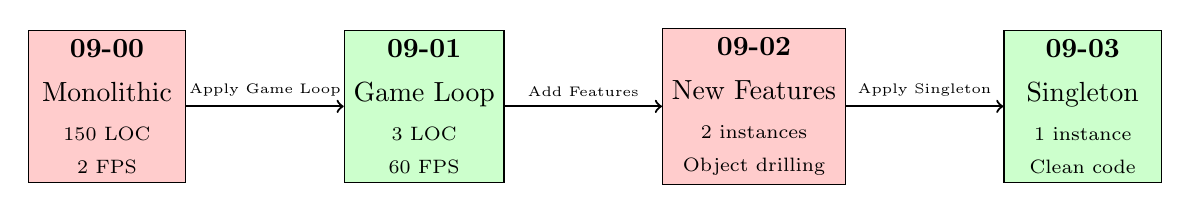
\begin{tikzpicture}[node distance=2cm]
                \node[rectangle, draw, fill=red!20, minimum width=2cm, minimum height=1.5cm, align=center] (b00) {
                    \textbf{09-00} \\[4pt]
                    Monolithic \\[2pt]
                    \scriptsize 150 LOC \\
                    \scriptsize 2 FPS
                };

                \node[rectangle, draw, fill=green!20, minimum width=2cm, minimum height=1.5cm, align=center, right=of b00] (b01) {
                    \textbf{09-01} \\[4pt]
                    Game Loop \\[2pt]
                    \scriptsize 3 LOC \\
                    \scriptsize 60 FPS
                };

                \node[rectangle, draw, fill=red!20, minimum width=2cm, minimum height=1.5cm, align=center, right=of b01] (b02) {
                    \textbf{09-02} \\[4pt]
                    New Features \\[2pt]
                    \scriptsize 2 instances \\
                    \scriptsize Object drilling
                };

                \node[rectangle, draw, fill=green!20, minimum width=2cm, minimum height=1.5cm, align=center, right=of b02] (b03) {
                    \textbf{09-03} \\[4pt]
                    Singleton \\[2pt]
                    \scriptsize 1 instance \\
                    \scriptsize Clean code
                };

                \draw[->,thick] (b00) -- (b01) node[midway,above,font=\tiny] {Apply Game Loop};
                \draw[->,thick] (b01) -- (b02) node[midway,above,font=\tiny] {Add Features};
                \draw[->,thick] (b02) -- (b03) node[midway,above,font=\tiny] {Apply Singleton};
            \end{tikzpicture}
        }
    \end{center}

    \vspace{0.5cm}

    \begin{block}{Key Takeaways}
        \begin{itemize}
            \item Design patterns solve \textbf{real problems}
            \item Software evolves → problems emerge → patterns help
            \item \textbf{Maintain solutions} while solving new problems
            \item Always consider \textbf{trade-offs}
        \end{itemize}
    \end{block}
\end{frame}

\begin{frame}{Comparison Table}
    \begin{center}
        \small
        \begin{tabular}{|l|c|c|c|c|}
            \hline
            \textbf{Aspect} & \textbf{09-00} & \textbf{09-01} & \textbf{09-02} & \textbf{09-03} \\
            \hline
            FPS & 2 & 60 & 60 & 60 \\
            \hline
            Main LOC & 150+ & 3 & 32 & 3 \\
            \hline
            Testability & 0\% & 100\% & 100\% & 100\% \\
            \hline
            Flickering & Yes & No & No & No \\
            \hline
            Instances & - & - & 2+ & 1 \\
            \hline
            Drilling & - & - & 4 levels & 0 \\
            \hline
            HUD Score & - & - & Wrong & Correct \\
            \hline
            Params & - & - & 6 & 0 \\
            \hline
        \end{tabular}
    \end{center}

    \vspace{0.5cm}

    \begin{exampleblock}{Achievement}
        From \textbf{2 FPS monolith} to \textbf{60 FPS professional architecture}! 🎉
    \end{exampleblock}
\end{frame}

% ============================================================================
% SECTION 9: DISCUSSION
% ============================================================================
\section{Discussion Questions}

\begin{frame}{Discussion Questions}
    \begin{block}{Game Loop Pattern}
        \begin{enumerate}
            \item Why does separating update/draw solve flickering?
            \item How does delta time ensure consistent speed?
            \item Why is testability important for games?
            \item What happens if update() takes $>$ 16ms?
        \end{enumerate}
    \end{block}

    \begin{block}{Singleton Pattern}
        \begin{enumerate}
            \setcounter{enumi}{4}
            \item What prevents multiple GameManager instances?
            \item Why is getInstance() static?
            \item When should you NOT use Singleton?
            \item How is Singleton different from static class?
        \end{enumerate}
    \end{block}
\end{frame}

\begin{frame}{Design Thinking Questions}
    \begin{block}{Critical Thinking}
        \begin{enumerate}
            \setcounter{enumi}{8}
            \item Could we solve object drilling WITHOUT Singleton?
            \item What are trade-offs of Dependency Injection?
            \item Why didn't 09-00 need Singleton?
            \item How do you decide when to apply a pattern?
        \end{enumerate}
    \end{block}

    \vspace{0.5cm}

    \begin{exampleblock}{Remember}
        \textbf{Patterns are tools, not rules!} \\
        Understand the problem first, then choose the right solution.
    \end{exampleblock}
\end{frame}

% ============================================================================
% SECTION 10: ASSESSMENT
% ============================================================================
\section{Assessment}

\begin{frame}{Assessment Rubric}
    \begin{center}
        \small
        \begin{tabular}{|l|p{3cm}|p{3cm}|p{3cm}|}
            \hline
            \textbf{Criteria} & \textbf{Basic} & \textbf{Proficient} & \textbf{Advanced} \\
            \hline
            Understanding & Explains patterns & Compares branches & Analyzes trade-offs \\
            \hline
            Implementation & Compiles correctly & Works correctly & Optimized \\
            \hline
            Testing & Basic tests & Full coverage & Edge cases \\
            \hline
            Documentation & Code comments & Clear docs & Teaching quality \\
            \hline
        \end{tabular}
    \end{center}

    \vspace{0.5cm}

    \begin{block}{Practical Exercise}
        \begin{itemize}
            \item Implement a new feature (e.g., player lives)
            \item Choose appropriate pattern (Singleton or not?)
            \item Justify your design decision
            \item Write tests
        \end{itemize}
    \end{block}
\end{frame}

\begin{frame}{Learning Outcomes}
    \textbf{After completing Week 09, students should be able to:}

    \begin{itemize}
        \item[\faCheckCircle] Implement proper game loop with delta time
        \item[\faCheckCircle] Explain frame-rate independent movement
        \item[\faCheckCircle] Write testable game logic
        \item[\faCheckCircle] Implement Singleton pattern correctly
        \item[\faCheckCircle] Identify when to use (and not use) patterns
        \item[\faCheckCircle] Analyze design trade-offs
        \item[\faCheckCircle] Debug state management issues
        \item[\faCheckCircle] Apply patterns to new problems
    \end{itemize}

    \vspace{0.5cm}

    \begin{exampleblock}{Industry Readiness}
        These skills are \textbf{essential} for professional game development!
    \end{exampleblock}
\end{frame}

% ============================================================================
% CLOSING
% ============================================================================
\begin{frame}{Resources}
    \begin{block}{Repository}
        All code, diagrams, and documentation available at: \\
        \texttt{rpg/} directory with branches:
        \begin{itemize}
            \item \texttt{09-00-without-game-loop}
            \item \texttt{09-01-with-game-loop}
            \item \texttt{09-02-without-singleton}
            \item \texttt{09-03-with-singleton}
            \item \texttt{09-04-analysis}
        \end{itemize}
    \end{block}

    \begin{block}{Documentation}
        \begin{itemize}
            \item \texttt{docs/09-00-problem.md}
            \item \texttt{docs/09-01-solution.md}
            \item \texttt{docs/09-02-problem.md}
            \item \texttt{docs/09-03-solution.md}
            \item \texttt{docs/WEEK-09-OVERVIEW.md}
        \end{itemize}
    \end{block}
\end{frame}

\begin{frame}[standout]
    \Huge Thank You!

    \vspace{1cm}

    \Large Questions?

    \vspace{1cm}

    \normalsize
    \textbf{Remember:} \\
    Perfect is the enemy of good. \\
    Start simple, improve iteratively, \\
    apply patterns when needed!
\end{frame}

\end{document}
